\section{Funktionelle krav}\label{funktionellekrav}
\textit{For at sikre systemets funktionalitet i forhold til ovenstående løsningsstrategi opstilles en række funktionelle krav for hele systemet. Disse krav danner grundlag for efterfølgende indhold i kapitlet. Der opstilles ydermere et blokdiagram for at give et overblik kravene til systemet.}

Formålet med systemet er, at udvikle en aktivitetsmåler som har potentialet til at reducere antallet af inaktive børn i aldersgruppen 9-12 år. Dette gøres med henblik på at ændre den teknologiske udviklings påvirkning af børns aktivitetsvaner fra inaktivitet til aktivitet.
Der ønskes et system som detekterer aktiviteterne gang, løb og cykling, da disse er gængse aktiviteter i et barns hverdag. Detekteringen af disse aktiviteter kan ske gennem et accelerometer og og et gyroskop, hvorefter systemet, gennem algoritmer, skal kunne adskille gang, løb og cykling.
Intensiteten af aktiviteterne registreres igennem puls, da dette giver en indikation af det fysiologiske udbytte, barnet får ud af en given aktivitet. Det vil være væsentligt at sommenholde puls og tid, da det anbefales at børn skal være aktve 30 minutter med høj intensitet mindst tre gange om ugen. Derudover er barnets kognitive funktion, som følge af fysisk aktivitet i 11-20 minutter, øget i 50 minutter.

For at systemet har en motiverende effekt på børn, skal der være en brugerflade som børnene finder interessant. Denne skal visuelt give feedback på dagens samlede præstationer samt progressionen i aktivitetsniveauet.

Systemet skal detektere børns aktivitet igennem en hel dag, uden at være til gene, hvormed det skal fungere uafhængigt af andre systemer. Det skal derfor være et trådløst system, som kan sende data til en ekstern enhed og er batteridrevet med mindst en dags levetid. Derudover skal det være elektrisk sikkert, således at barnet ikke kan komme til skade som følge af aktivitetsmålerens design. 

På baggrund af ovenstående, udformes de funktionelle krav således at systemet skal: 
\begin{itemize}
	\item Gennem sensorer kunne detektere aktiviteterne gang, løb og cykling.
	\item Gennem algoritmer i softwaren kunne adskille gang, løb og cykling.
	\item Kunne registrere intensiteten af de givne aktiviteter igennem puls.
	\item Være komfortabelt, hvorfor det trådløst skal kunne videresende signaler til en ekstern enhed og være batteridrevet over en hel dag.
	\item Være elektrisk sikkert for brugeren.
	\item I den eksterne enhed, behandle og repræsentere signalerne visuelt som intensiteten af en aktivitet i forhold til tid.
	\item Motivere børn i aldersgruppen 9-12 år. 
\end{itemize}

\subsection{Blokdiagram}
Ud fra de kravene til systemet, udformes et blokdiagram, som illustreres på \figref{fig:blokdiagram}. På denne fremgår rækkefølgen af blokkene samt om de er analoge eller digitale. 

Den analoge del, som er omringet af en rød firkant på \figref{fig:blokdiagram}, består af inputs fra de tre analoge\fxnote{var de ikke digitale} sensorer; accelerometer, gyroskop og pulssensor. Disse analoge inputs konverteres fra analoge til digitale signaler gennem en ADC. Herefter skal signalerne i den digitale del i slaven adskilles så der kan registreres hvor vidt barnet går, løber eller cykler. Gennem trådløs kommunikation mellem de to digitale dele, overføres data til mater, hvor det behandles. Sidst visualiseres dataet, så børnene kan se i hvor lang tid de har udførst en given aktivitet.  

 \begin{figure}[H]
 	\centering
 	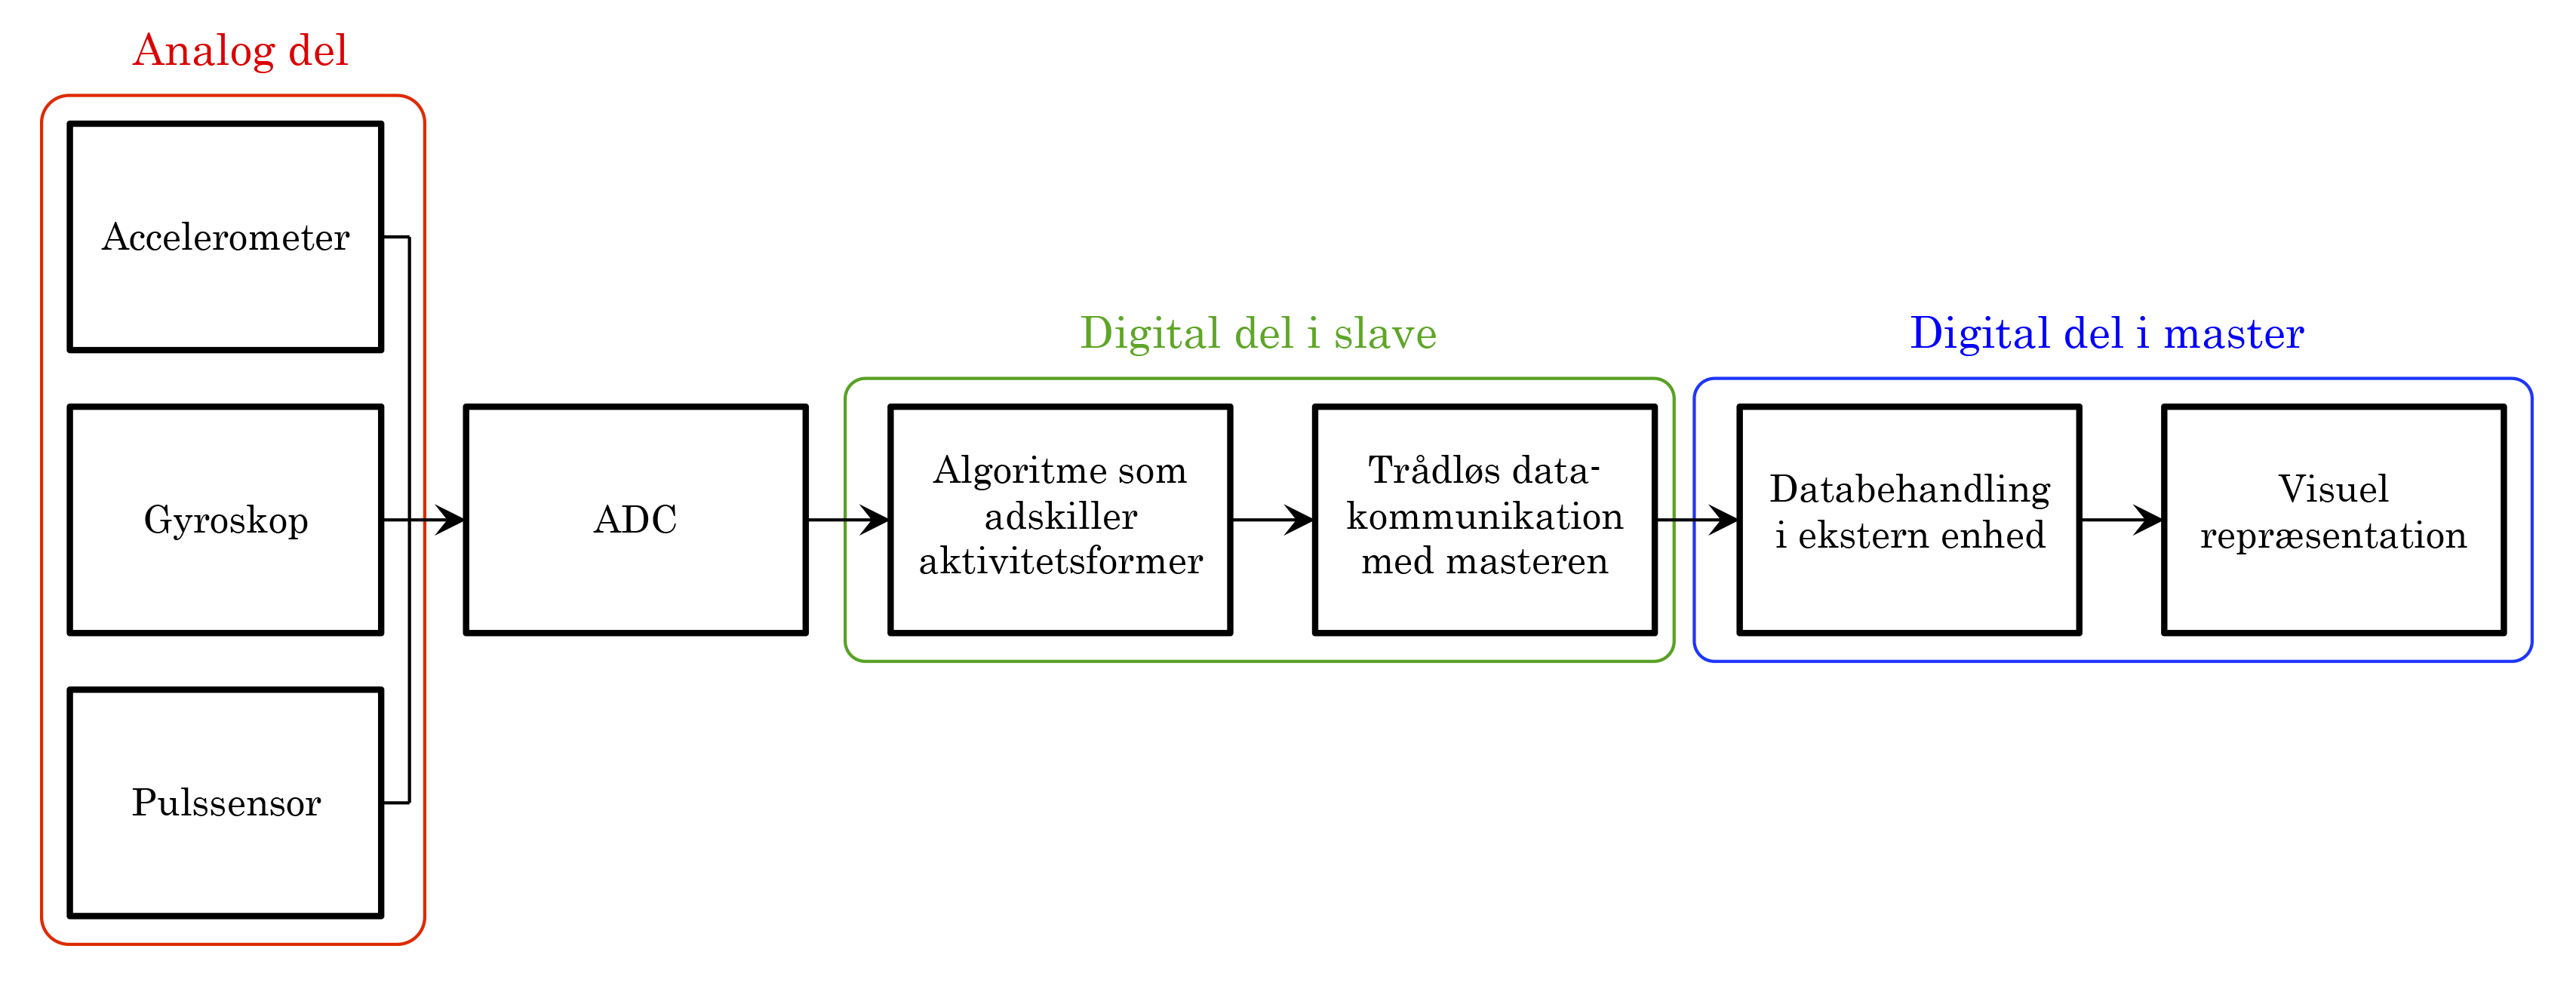
\includegraphics[scale=0.54]{figures/bProblemloesning/blokdiagram2.png}
 	\caption{Blokdiagram for systemet, som opdeles i den analoge del, og de to digitale dele. Den analoge del er omkranset med en rød firkant, slaven er omkranset med en grøn firkant og master er omkranset med en blå firkant.}
 	\label{fig:blokdiagram}
 \end{figure}